\section*{Results}
\subsection{Prediction Gain}
For the purpose of testing LP prediction gain (PG) shown in \autoref{eq:PG} will be used. 
\begin{equation}\label{eq:PG}
PG = 10 log_{10}\bigg(\frac{\sigma^2_x}{\sigma^2_\varepsilon}\bigg) = 10 log_{10}\bigg(\frac{E\{x^2[n]\}}{E\{\varepsilon^2[n]\}}\bigg)
\end{equation}
where PG is the ratio between the variance of the input signal $x[n]$ and the variance of the prediction error $\varepsilon$ in (dB). The higher the PG the better the prediction is.



\subsection{Determining System Parameters}
The parameters which should be detemined are $fs$, $P$, $N$, $O$, and $M$ using \autoref{eq:PG}.         
The PG of variable $fs$ is shown on \autoref{fig:fsPredict}.

\begin{figure}[H]
	\centering
	\textbf{\textit{Here is going to be a graph of PG determined by fs}}
	\caption{PG }
	\label{fig:fsPredict}
\end{figure}


%These are detemined respectively using a Prediction Gain ($PG$) to find the optimum value. 
The PG of variable $N$, $O$ and $M$ is seen on \autoref{fig:PredictParameters}. 
\begin{figure}[H]
	\centering
	\textbf{\textit{Here is going to be a graph of PG determined by N}}
	\textbf{\textit{Here is going to be a graph of PG determined by O}}
	\textbf{\textit{Here is going to be a graph of PG determined by M}}
	\caption{PG }
	\label{fig:PredictParameters}
\end{figure}

\subsection{Simulation of Feedforward LP FXLMS}

\begin{figure}[H]
	\centering
	\tikzsetnextfilename{DelayRatio}
	% This file was created by matlab2tikz.
%
%The latest updates can be retrieved from
%  http://www.mathworks.com/matlabcentral/fileexchange/22022-matlab2tikz-matlab2tikz
%where you can also make suggestions and rate matlab2tikz.
%
\definecolor{mycolor1}{rgb}{0.00000,0.44700,0.74100}%
\definecolor{mycolor2}{rgb}{0.85000,0.32500,0.09800}%
%
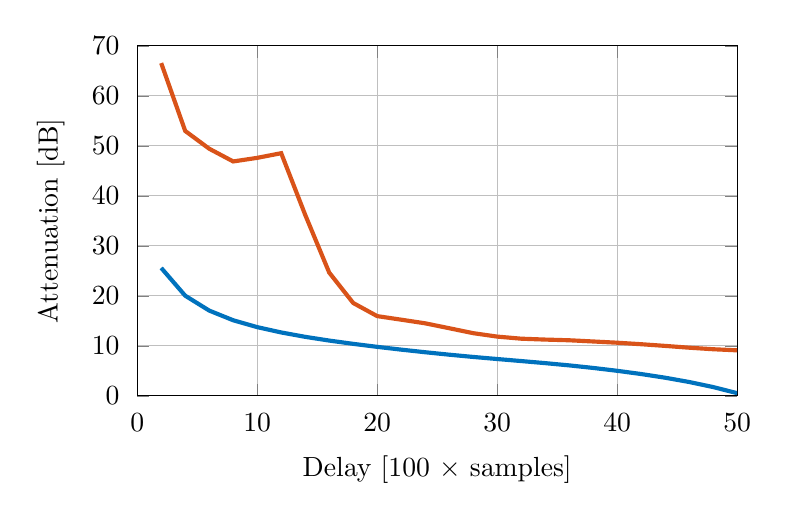
\begin{tikzpicture}

\begin{axis}[%
width=3in,
height=1.75in,
scale only axis,
xmin=0,
xmax=50,
xmajorgrids,
xlabel={Delay [100 $\times$ samples]},
ymin=0,
ymax=70,
ylabel style={yshift=0.3em},
xlabel style={yshift=-0.2em},
ytick={0,10,...,70},
ymajorgrids,
ylabel={Attenuation [dB]},
xticklabel shift={.1cm},
yticklabel shift={.1cm},
axis background/.style={fill=white}
]
\addplot [color=mycolor2,solid,line width=1.5pt,forget plot]
  table[row sep=crcr]{%
2	66.5420250310586\\
4	52.9717264302022\\
6	49.4175149424998\\
8	46.8717703569681\\
10	47.5886347675082\\
12	48.5221420089092\\
14	36.1913078215459\\
16	24.6480360536532\\
18	18.5625963047043\\
20	15.9345988709594\\
22	15.2225924490026\\
24	14.4941735350858\\
26	13.5145912190769\\
28	12.5242379572864\\
30	11.8400523957144\\
32	11.4203165228037\\
34	11.2428861871564\\
36	11.1050592495872\\
38	10.862823901561\\
40	10.6158645117455\\
42	10.3154480278615\\
44	9.97867799972119\\
46	9.61958031033587\\
48	9.31052791122033\\
50	9.08997582022533\\
};
\addplot [color=mycolor1,line width=1.5pt,solid,forget plot]
table[row sep=crcr]{%
	2	25.5751628128288\\
	4	20.0199680852144\\
	6	17.0442763613153\\
	8	15.1060127156582\\
	10	13.7310612019933\\
	12	12.6685774343164\\
	14	11.7903474171974\\
	16	11.0441690144364\\
	18	10.3883064900616\\
	20	9.78797702825996\\
	22	9.23075404560805\\
	24	8.7110676592604\\
	26	8.22176906503967\\
	28	7.77006791263877\\
	30	7.35426684398216\\
	32	6.94907270624338\\
	34	6.5323972441528\\
	36	6.08060777493347\\
	38	5.57101511941803\\
	40	4.99733350616245\\
	42	4.35167702165293\\
	44	3.61433096515684\\
	46	2.757705271237\\
	48	1.74470077738877\\
	50	0.5254168140125\\
};
\end{axis}
\end{tikzpicture}%
	\caption{Attenuation achieved by the system for different system delays.}
	\label{Fig:Reference to noise ratio}
\end{figure}








% At this point in time all results are not yet certain, however we will give an idea of how they are going to turn out.
% As presented in the paper thus far, we know what kind of noise we would like to cancel out and how we want to do it. The following list tells which graph will be used to show the results of the acceptance tests.

% \begin{itemize}
% \item Prediction gain - The difference between the input signal and the estimated signal, measured in dB. Used in the LP part.
% \item A plot comparison of frequency response between: A pure signal, a signal with FXLMS noise attenuation and a signal with LP combined with FXLMS attenuation
% \item An expansion of \autoref{Fig:Reference to noise ratio}: As of now only attenuation is showed, but in the future another graph in the figure will show the attenuation of the FXLMS combined with LP - which should yield better attenuation at larger delays.

% \end{itemize}




%\vspace{5in}